\chapter{Introduction}
\label{chap:introduction}

\vspace{1cm}

Created by John Gruber in 2004, with extensive help by the late Aaron Swartz, Markdown is a markup language which allows its users to format
text using a syntax which focuses on readability and simplicity.
Drawing inspiration from previously existing markup languages that were used on email and usenet clients, such as reStructuredText and Textile,
and inspired by Aaron Swartz's recently created markup language named ``atx'', John Gruber created two things: the syntax for the language, and a simple
Perl script (``Markdown.pl'') which replaces the markers for that language with HTML tags.\footcite{gruber2004markdown}\newline

Since its inception, Markdown became wildly popular and is an accepted and adopted format in many popular websites and tools. It is now used for
numerous different use-cases, such as reproductible scientific research, documentation (technical or not), website templating, organization
methodologies (such as ``second brain''), and many others. This means that while simplistic in nature, Markdown has inspired troves of
new projects which help people daily.\newline

\begin{figure}[H]
    \hspace{-3cm}
    \subfloat[\centering Markdown code snippet before interpretation]{{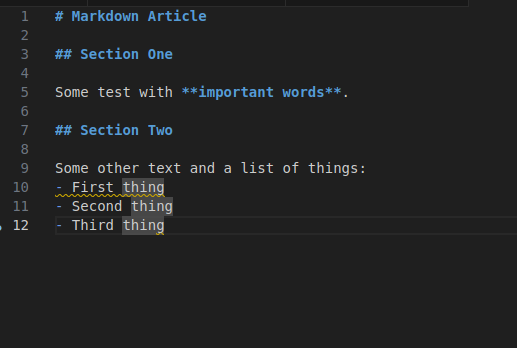
\includegraphics[width=9.5cm]{before} }}
    \qquad
    \subfloat[\centering Markdown output after interpretation]{{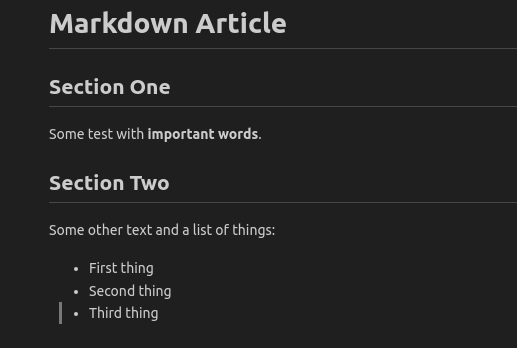
\includegraphics[width=9.5cm]{after} }}
    \caption{Markdown, before and after.}
    \label{fig:example-simple-syntax}
\end{figure}

Figure \ref{fig:example-simple-syntax} features a ``before and after'' view of 3 base Markdown features: headings (denoted by the `\#' tags),
bold text (indicated by `**' markers), and lists (items preceded by dashes). Thanks to its readability and syntax highlighting, seasoned
Markdown users know instinctively what the output after interpretation will be.\newline

However, on more complex examples, this instinctive feeling disappears as several aspects may come into play: what kind of Markdown variant will
be used, what implementation is used to interpret and output the corresponding HTML, and possible incompatibilities when migrating Markdown files
from one tool to the other due to the two previous factors. Even when a user knows what the output will look like, the underlying HTML code
will differ quite a lot from implementation to implementation.\newline

This article aims to explore the origins of markup languages in general, the role and influence of Markdown (and its many variants)
in various fields, and address the issues arising from the lack of standardization of this markup language.